\documentclass[compress]{beamer}

\usepackage[utf8]{inputenc}
\usepackage{amssymb}
\setbeamertemplate{caption}{\raggedright\insertcaption\par}

\usetheme[navigation]{UMONS}
%\usetheme[navigation, no-subsection, no-totalframenumber]{UMONS}

\newcommand{\IR}{\mathbb{R}}


\title{Bandwidth estimation : metrics, measurement techniques, and tools}
\author{M. Lempereur \\
J. Gheysen}
\institute[(Info)]{%
  Département d'Informatique\\
  Université de Mons
  \\[2ex]
  
\includegraphics[height=4ex]{UMONS}\hspace{2em}%
  \raisebox{-1ex}{
\includegraphics[height=6ex]{UMONS_FS}}
}

\begin{document}

\begin{frame}[plain]
  \titlepage
\end{frame}

\begin{frame}
  \tableofcontents
\end{frame}

\section{Introduction}
\begin{frame}{Introduction}

\end{frame}

%%%%%%%%%%%%%%%%%%%%%%%%%%%%%%%%%%%%%%%%%%%%%%%%%%%%%%%%%%%%%%%%%%%%%%%%
%Dans l'utilisation quotidienne beaucoup de termes sont
%confondus, le but ici est de formaliser la définition autour
%de la vitesse d'une connection et de la "bande passante".
%D'apporter des mesures précises et de faire le point sur les
%technologies existantes à ce niveau. 
%%%%%%%%%%%%%%%%%%%%%%%%%%%%%%%%%%%%%%%%%%%%%%%%%%%%%%%%%%%%%%%%%%%%%%%%

\begin{frame}{Introduction}{Vocabulaire 1/2}
	\begin{figure}
   		\begin{minipage}[c]{.46\linewidth}
   			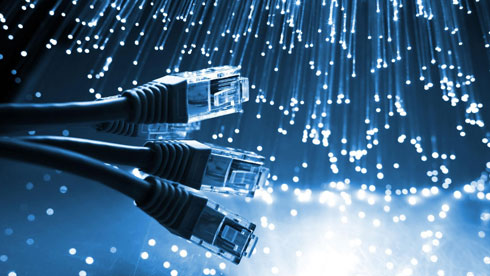
\includegraphics[scale=0.23]{capacity.JPG}
   			\caption{Capacité}
   		\end{minipage} \hfill
   		\begin{minipage}[c]{.46\linewidth}
      		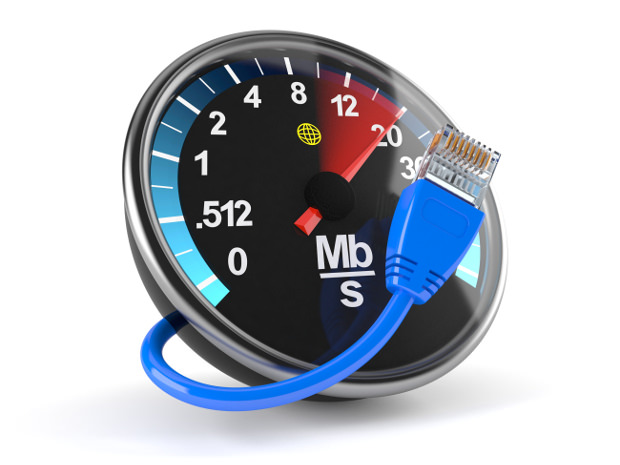
\includegraphics[scale=0.18]{bande_passante.jpg}
      		\caption{Bande Passante}
   		\end{minipage}
   		\begin{minipage}[c]{.46\linewidth}
   			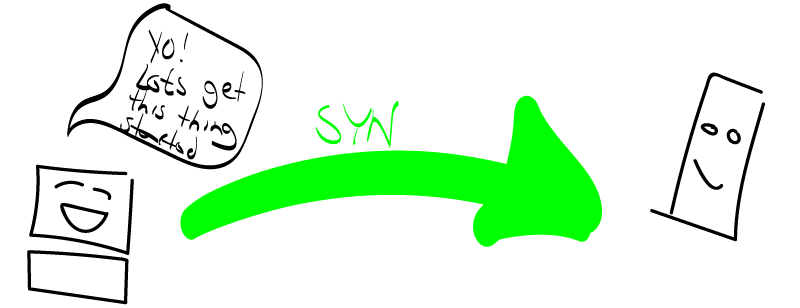
\includegraphics[scale=0.2]{tcp.png}
   			\caption{Bulk-Transfert-Capacity}
   		\end{minipage} \hfill
	\end{figure}
\end{frame}

\begin{frame}{Introduction}{Vocabulaire 2/2}
\begin{itemize}
	\item Différenciation entre liens de la couche données (1) et couche IP(2).
	\begin{enumerate}
		\item \textbf{Segment} : Lien physique point à point. %Etendre aux autres points dans l'article ?
		\item \textbf{Hop} (saut) : Consiste en un ensemble de segments. %Connectés à travers switchs/bridges...
	\end{enumerate}
	\vspace{10pt}
	\item \textbf{Chemin end-to-end} : Lie un hôte à une source via une suite de hops.
	\vspace{10pt}
	\item Que mesurer ? Dans quelle situation ? 
	\begin{itemize}
		\item \textbf{Lien unique (hop)} : Capacité, Bande Passante.
		\item \textbf{Chemin} : Capacité, Bande Passante, Bulk-Transfert-Capacity.
	\end{itemize}
\end{itemize}
\end{frame}

%%%%%%%%%%%%%%%%%%%%%%%%%%%%%%%%%%%%%%%%%%%%%%%%%%%%%%%%%%%%%%%%%%%%%%%%
%Tout d'abord != entre lien et chemin (= ensemble de liens)
%ATTENTION : UN SEGMENT est en réalité une FRAME (layer 2).
%Ici nous utilisons lien pour donner définition globale.
%Capacité : Valeur maximale du flux pouvant traverser un lien,
%càd quantité maximale de bits pouvant transiter à travers
%le lien par unité de temps. 
%Bande passante disponible : Capacité du lien non utilisée,
%alors utilisable afin d'écouler du traffic. 
%BTC : Représente le débit atteignable par une seule 
%connexion TCP. 
%%%%%%%%%%%%%%%%%%%%%%%%%%%%%%%%%%%%%%%%%%%%%%%%%%%%%%%%%%%%%%%%%%%%%%%%


\section{Données mesurées}
\subsection{Capacité}
\begin{frame}{Capacité}
	Posons :
	\begin{itemize}
	\item $C_{L2}$ la capacité nominale du \textbf{segment},
	\item $L_{L3}$ la taille du paquet IP, 
	\item $H_{L2}$ l'overhead de la couche 2. 
	\end{itemize}
	\begin{block}{Temps de transmission : $\Delta_{L3}$}
		$$\Delta_{L3} = \frac{L_{L3} + H_{L2}}{C_{L2}}$$
	\end{block}
	\begin{block}{Capacité couche IP:  $C_{L3}$}
		$$C_{L3} = \frac{L_{L3}}{\Delta_{L3}} = \frac{L_{L3}}{\frac{L_{L3}+H_{L2}}{C_{L2}}} = C_{L2} \frac{1}{1+\frac{H_{L2}}{L_{L3}}}$$
	\end{block}
\end{frame}
%%%%%%%%%%%%%%%%%%%%%%%%%%%%%%%%%%%%%%%%%%%%%%%%%%%%%%%%%%%%%%%%%%%%%%%%
%Bien insister sur le fait qu'on regarde le paquet IP au 
%travers d'un SEGMENT. 
%La capacité C_L3 est donc directement proportionnelle à la 
%capacité de la couche d'en dessous et inversément proportionnelle
%au rapport Overhead/Longueur (Plus ce rapport est grand plus la 
%capacité est réduite. Ce dernier dépend du MTU (Maximum Transfert
%Unit) d'un paquet de la couche IP. 
%%%%%%%%%%%%%%%%%%%%%%%%%%%%%%%%%%%%%%%%%%%%%%%%%%%%%%%%%%%%%%%%%%%%%%%%

\begin{frame}
	\begin{alertblock}{Remarque}
		Le rapport $\frac{H_{L2}}{L_{L3}}$ est borné par le MTU (Maximum Transmission Unit).
	\end{alertblock}
\begin{figure}[hbtp]
\centering
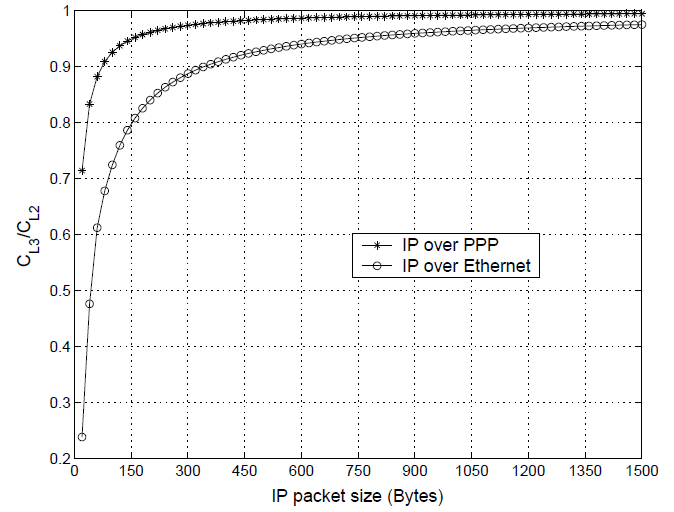
\includegraphics[scale=0.25]{schema1.PNG}
\caption{Rapport des capacités d'un segment délivré à la couche IP en fonction de sa taille.}
\end{figure}
		\begin{block}{Capacité sur un chemin}
		$$C = \min\limits_{i=1,...,H} C_{i}$$
		\end{block}
\end{frame}

%%%%%%%%%%%%%%%%%%%%%%%%%%%%%%%%%%%%%%%%%%%%%%%%%%%%%%%%%%%%%%%%%%%%%%%%
%En ce qui concerne le MTU : il définit un overhead fixe pour 
%une taille de paquet maximum => Remplir un max les paquets.
%Appelés datagrammes IP.
%Plus le paquet sera grand, plus le rapport sera petit et avantageux.   
%%%%%%%%%%%%%%%%%%%%%%%%%%%%%%%%%%%%%%%%%%%%%%%%%%%%%%%%%%%%%%%%%%%%%%%%

\subsection{Bande Passante}
\begin{frame}{Bande Passante}
	\begin{figure}[hbtp]
		\centering
		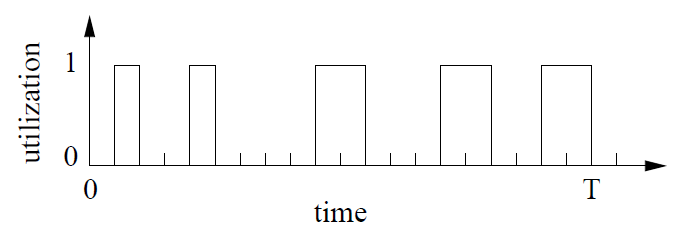
\includegraphics[scale=0.42]{schema2.PNG}
		\caption{Utilisation instantanée d'un lien durant un temps (0,T)}
	\end{figure}
	\begin{itemize}
		\item Utilisation du lien non-constante,
		\item Posons $u_i$ l'utilisation moyenne. 
	\end{itemize}
	\begin{block}{Bande passante disponible en moyenne : $A_{i}$}
		$$ A_i = (1 - u_i) C_i $$
	\end{block}
\end{frame}

%%%%%%%%%%%%%%%%%%%%%%%%%%%%%%%%%%%%%%%%%%%%%%%%%%%%%%%%%%%%%%%%%%%%%%%%
%A un temps donné, le lien transmet un paquet à sa full capacité (1) ou 
%est inutilisé. La formule donnée pour A_i comprend la bande passante 
%pour un seul hop i. 
%%%%%%%%%%%%%%%%%%%%%%%%%%%%%%%%%%%%%%%%%%%%%%%%%%%%%%%%%%%%%%%%%%%%%%%%

\begin{frame}
	\begin{block}{Bande passante sur un chemin}
		$$A = \min\limits_{i=1,...,H} A_{i}$$
	\end{block}
	\begin{alertblock}{Remarque}
		Bande passante et capacité ne sont pas toujours limitées sur le même lien. 
	\end{alertblock}
	\begin{figure}[hbtp]
		\centering
		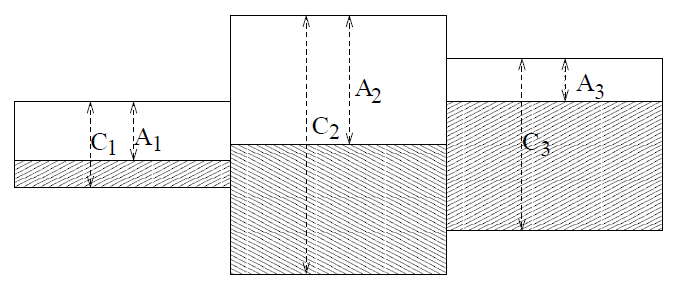
\includegraphics[scale=0.42]{schema3.PNG}
		\caption{Exemple de trafic pour un chemin de 3 hops}
	\end{figure}
	
\end{frame}

%%%%%%%%%%%%%%%%%%%%%%%%%%%%%%%%%%%%%%%%%%%%%%%%%%%%%%%%%%%%%%%%%%%%%%%%
%La bande passante disponible sur un chemin est le minimum de celle 
%dispo sur tous les liens de son chemin. 
%Dans l'exemple, la limitation se fait en 1 pour la capacité et en 3
%pour la bande passsante. 
%Ces calculs supposent que l'utilisation des liens est constante,
%cette assomption reste raisonnable pour des intervalles de temps 
%cours mais /!\ à la sporadicité et à la != diurne/nocturne, etc...
%Or ce n'est pas le cas, il faut donc effectuer des mesures rapides
%si on veut un aperçu en temps réel (utile pour certaines applis). 
%%%%%%%%%%%%%%%%%%%%%%%%%%%%%%%%%%%%%%%%%%%%%%%%%%%%%%%%%%%%%%%%%%%%%%%%

\subsection{Bulk-Transfert-Capacity}
\begin{frame}{Bulk-Transfert-Capacity (BTC)}
	\begin{alertblock}{Définition}
		Débit atteignable par une unique connection TCP en prenant compte du contrôle de congestion.
	\end{alertblock}
	Éléments influençant le flux TCP : 
	\begin{itemize}
		\item Taille des paquets transférés,
		\item Trafic croisé avec d'autres connections,
		\item Taille des buffers des sockets,
		\item Taille de la fenêtre de congestion,
		\item ...
	\end{itemize}
\end{frame}

%%%%%%%%%%%%%%%%%%%%%%%%%%%%%%%%%%%%%%%%%%%%%%%%%%%%%%%%%%%%%%%%%%%%%%%%
%Représente 90% du trafic
%Beaucoup de facteurs influençant : transfert size, cross-traffic, 
%competiting TCP connections, TCP socket buffer size, congestion, 
%variations liées à l'implémentation,...
%Pour une page Web : congestion window, RTT, slow-start mechanism
%TODO Regarder avec l'histoire de capacité C/2. 
%%%%%%%%%%%%%%%%%%%%%%%%%%%%%%%%%%%%%%%%%%%%%%%%%%%%%%%%%%%%%%%%%%%%%%%%

\section{Techniques de mesure}
\begin{frame}{Techniques de mesure}

\end{frame}

\section{Taxonomie des outils de mesure}
\begin{frame}{Taxonomie des outils de mesure}

\end{frame}


\end{document}
%%% Local Variables: 
%%% mode: latex
%%% TeX-master: t
%%% End: 
\grid
